\clearpage

\def\chaptertitle{System Implementation}

\lhead{\emph{\chaptertitle}}

\chapter{\chaptertitle}
\label{ch:experimental-setup}

Based on the previous high-level overview of the architectures and algorithms involved, in this chapter we will first discuss the micro-service application architecture used to test the auto-scaling on, along with its features in section \ref{sec:ch4-microservice-overview}. With this background, section \ref{sec:ch4-data-generation} will give an explanation of the workload generator bundled along with the micro-service deployment, and how that was used to generate the time-series workload typically seen in edge deployments. Finally, we will discuss the technical configurations of the hybrid autoscaler itself in section \ref{sec:ch4-hybrid-auto-arch}. This will involve how the workload information is communicated between cloud and edge layers, how the autoscaler parameters for both reactive and proactive subsystems are configured, and how the forecaster is configured to use the time-series data to generate forecast values for a sufficiently large time-period to minimize training times even further. Finally, the hyper-parameter tuning configured by the autoscaler controller will be further elaborated.

\section{Micro-service Overview}
\label{sec:ch4-microservice-overview}

The container orchestration used for deploying the micro-service deployment, custom hybrid autoscaler, as well as all the additional telemtry tools was Kubernetes. Kubernetes offered the highest configurability for such a project, and combined with its ease-of-use, made it ideal for stress testing auto-scaling. DeathStarBench \footnote{\url{https://github.com/delimitrou/DeathStarBench/tree/master/socialNetwork}}, a social network micro-service implementation developed by Y. Gan et al. \cite{gan2019open} was purpose-built for conducting benchmarks on edge architectures with constraints such as SLA agreements, and was thus deployed on the Kubernetes platform. The application mimics a typical large-scale social network application and supports common actions such as registering and login for user credentials, creating user posts on their timeline, reading other user timelines, receiving follower recommendations, following and unfollowing of other users, and searching for users or posts. Figure \ref{fig:social-network-arch} shows the detailed architecture of the micro-service.\par

\begin{figure}[htb]
    \centering
    \caption{Social-Network Architecture, courtesy of Y. Gan et al. \cite{gan2019open}}
    \label{fig:social-network-arch}
    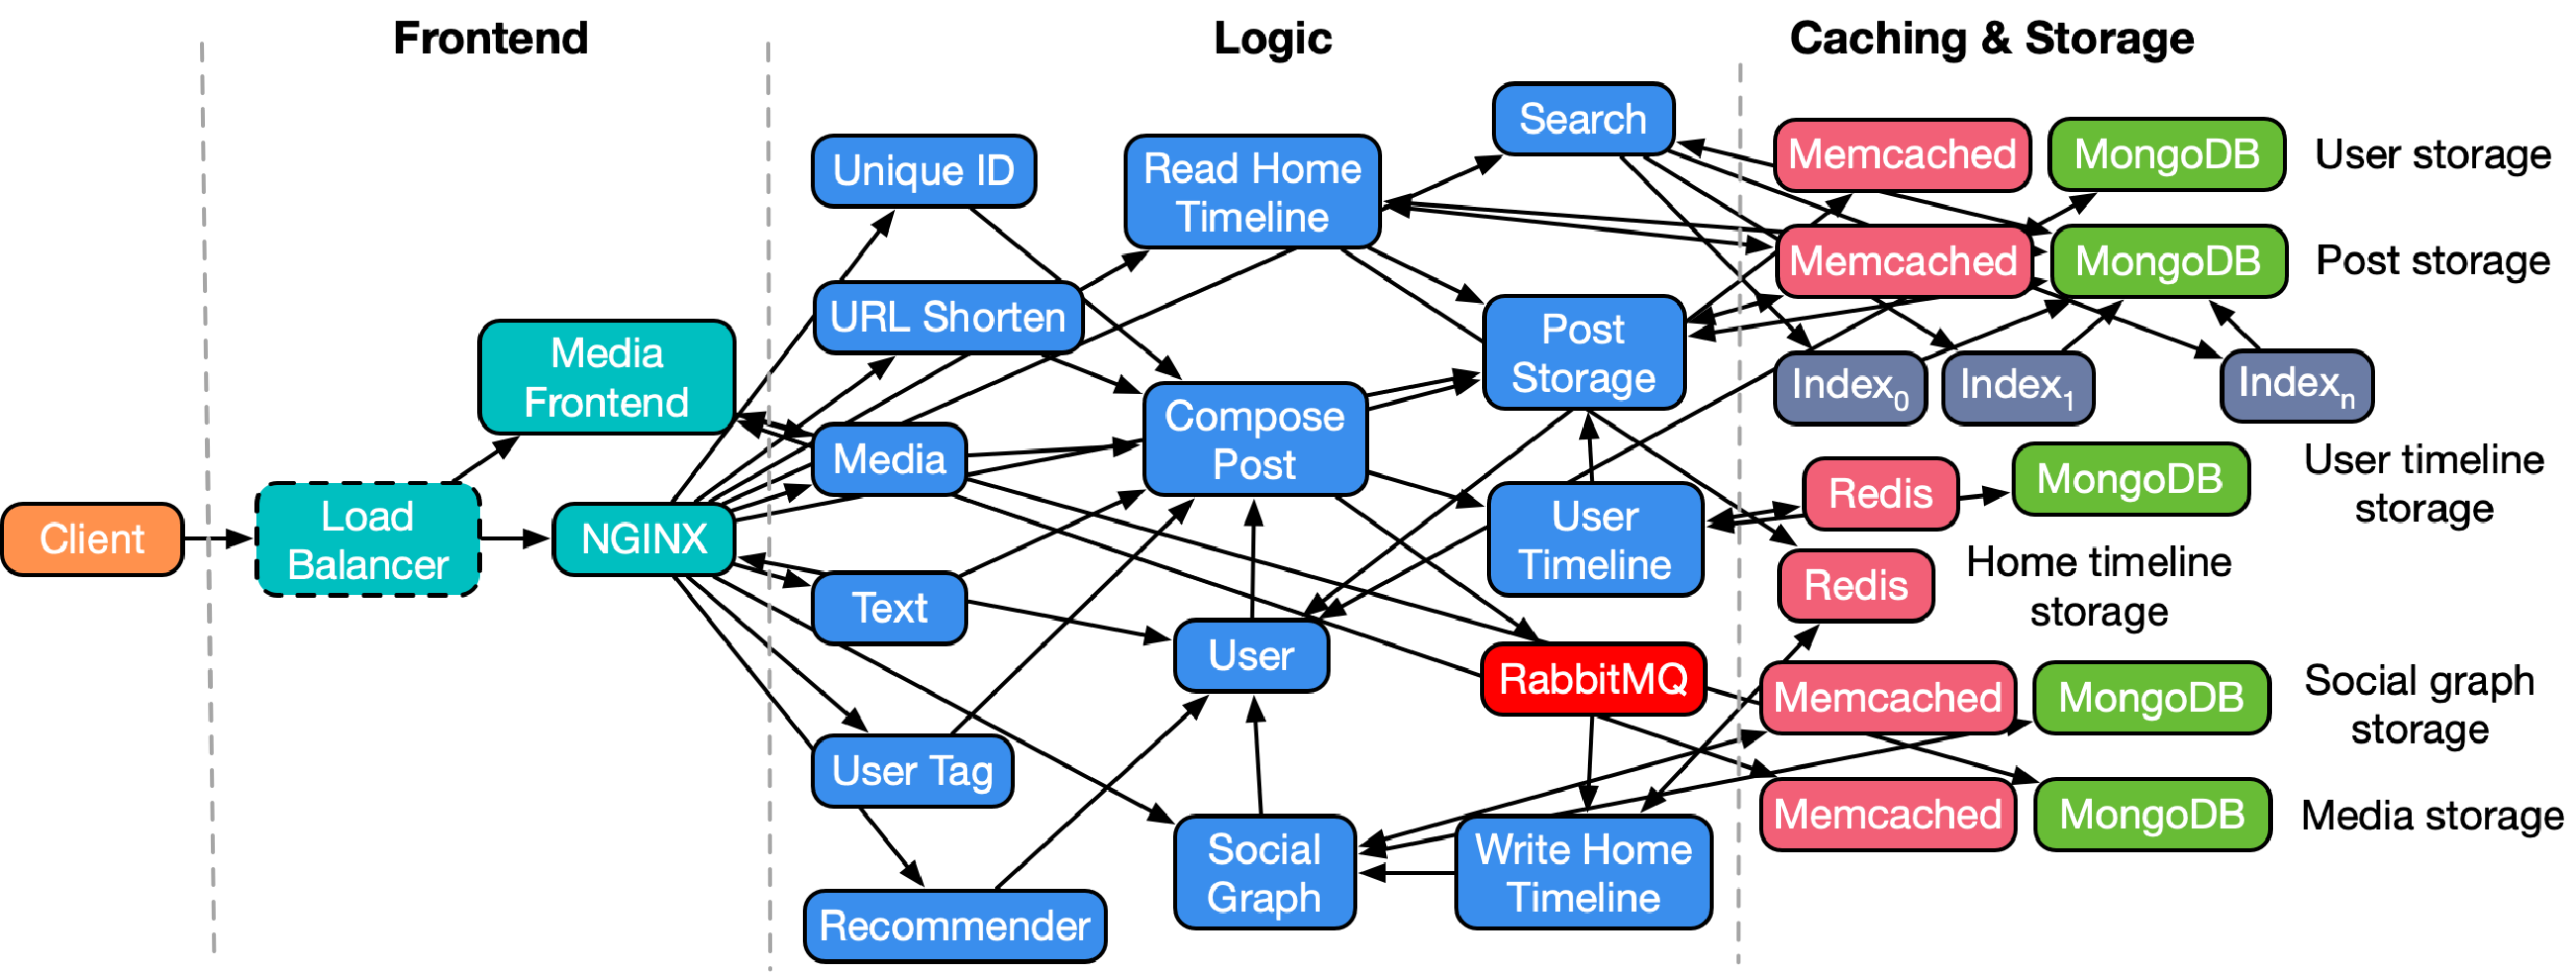
\includegraphics[width=1.0\linewidth]{Figures/Social-Network-Architecture.pdf}
\end{figure}

The end-to-end service implementation depicts a social network with a broadcast style approach. The user or client sends requests using HTTP to the front-end layer. These requests are processed using a load balancer implemented using an open-source deployment known as NGINX \footnote{\url{https://nginx.org/en/}}. NGINX then specifies the web server that has been selected, and communicates with the micro-services in the logic layer, which are responsible for composing and displaying the user and timeline posts. The logic layer also consists of micro-services for serving advertisements, search engines, and other capabilities commonly found in large scale applications. The search and advertisement engines are machine learning plugins capable of serving recommendations based on user interactions. The logic layer is capable of handling posts containing text, links, and media. Users can also mark other user's posts as favourites, re-post them, and reply to them privately or publicly. Users can also follow, unfollow, or block others. All these interaction results are stored in the storage layer, which uses memcached for caching results, and MongoDB for storing user profiles, posts, media, and recommendations in a persistent manner.

Users can sign in to the application website by connecting to the user interface deployment, which can be assigned a DNS address. For simplicity, in this experiment the DNS configuration was skipped in favour of exposing the Kubernetes cluster IP address of the front-end deployment, along with the social media application port. For example, an API request for reading user timelines will look as follows:\par

\begin{lstlisting}[
  caption={Social network API call template},
  captionpos=t,
  label={lst:social-network-api-template},
]
http://<app-IP>:<app-port>/wrk2-api/user-timeline/read
\end{lstlisting}

\section{Data Generation}
\label{sec:ch4-data-generation}

The social media deployment also comes with an HTTP workload generator, which
was leveraged to create a realistic simulation of a typical day of workload for the micro-service application. The generator, known as ``wrk2'', is an open-loop load generator. HTTP requests are sent out according to the user configuration, regardless of whether or not the responses of the previous requests have been received. This avoids issues such as queuing delays in the server, helping to maintain an even load throughout the generation process which aids in benchmark process. The workload generator supports a variety of load generation use-cases, as well as different APIs. For example, a POST request with a total load generation of 8 requests per second, using 2 parallel threads, with 5 open HTTP connections, and for a duration of 30 seconds looks as follows:\par

\begin{lstlisting}[
  caption={Workload generation example},
  captionpos=t,
  label={lst:workload-gen-example},
  language=bash
]
$ wrk2 -t2 -c5 -d30 -R8 http://<app-IP>:<app-port>/wrk2-api/post/compose
\end{lstlisting}

A typical IoT application in the edge has a semi-predictable workload pattern. What this means is that while the exact workloads may vary from day to day, the overall pattern of when the workloads peak and drop mostly remain constant from day to day. Tadakamalla and Menasc{\'e} \cite{tadakamalla2019characterization} demonstrated this through a survey of three popular IoT datasets. Their results demonstrated that IoT application workloads can be well approximated using a lognormal distribution. Furthermore, the authors also observed that the daily routines of the users greatly affected the workload patterns in the dataset. This information is used to inform our own workload generation, to inject predictable patterns in the hourly data.\par

\begin{figure}[htb]
    \centering
    \caption{IoT Data Characteristics, courtesy of Tadakamalla and Menasc{\'e} \cite{tadakamalla2019characterization}}
    \label{fig:iot-workload-characteristics}
    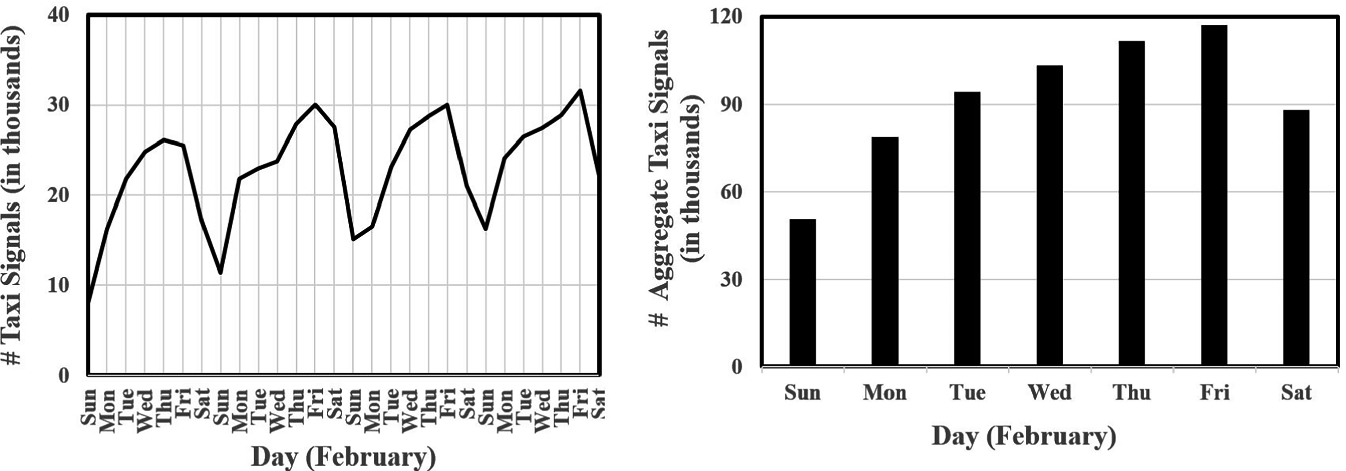
\includegraphics[width=1.0\linewidth]{Figures/IoT-Workload-Characteristics.png}
\end{figure}

In this experiment, it is assumed that the workload peaks in the morning and evening, while seeing moderate usage during the afternoon. The workload is lowest at night, maintaining a low usage throughout. The workload simulator was modified to introduce an element of randomness to mimic realistic weekly workloads, which can vary on occasions such as weekends and public holidays.\par

To achieve this, an IoT workload algorithm was created for leveraging the wrk2 generator to achieve this time-series. This is explained in algorithm \ref{alg:work-gen}. A constant light workload is set for night time consisting of six hours between 12:00am and 06:00 am, while different workloads for the eighteen different day time hours are set, with peaks set in the morning and evening, and dips in the afternoon. The algorithm also contains a small random ``offset'' variable to depict the randomness inherent in the workload. This is depicted using the function $\mathcal{F}$, where $\mathcal{F}(0,1)$ returns a random number between 0 and 1. This workload is then executed using the wrk2 generator to apply the HTTP load on the micro-service.

\begin{algorithm}
    \caption{IoT workload generation algorithm}
    \label{alg:work-gen}
    \begin{algorithmic}
        \State $offset \gets \alpha$
        \State $night\_workload \gets \omega$
        \State $day\_workload \gets [ \delta_1, \delta_2, ... , \delta_{18}]$
        \While{True}
            \For {i $\leftarrow$ 0 ... 6}
                \State $result \gets generate(night\_workload + \mathcal{F}(-offset,offset)$
            \EndFor
            \For {i $\leftarrow$ 0 ... 18}
                \State $result \gets generate(day\_workload[i] + \mathcal{F}(-offset,offset)$
            \EndFor
        \EndWhile
    \end{algorithmic}
\end{algorithm}

\section{Hybrid Autoscaler Configuration}
\label{sec:ch4-hybrid-auto-arch}

%In this section, the configuration parameters of the proposed hybrid autoscaler will be discussed. First, a brief background will be provided of how the social network application is connected to Kubernetes, so that it can send default and custom metrics such as application CPU usage and latency respectively. These custom metrics will then be discussed further, and how they are integrated for use in the horizontal pod autoscaler.\par

%With this background, a further discussion of the reactive subcomponent of the hybrid autoscaler is conducted, explaining its parameters and how it connects to the custom metrics API. The details of the proactive autoscaler are then discussed. This includes the architecture of the LSTM, default hyper-parameters, and the lookback and forecasting window. Finally, the autoscaler heuristic feedback will be discussed, including the exact parameters it modifies when it discovers an SLA violation.\par

With the Kubernetes container orchestration now installed on the servers, and the micro-service social network deployment set up on the orchestration platform, the hybrid autoscaler could be configured on the orchestration tool to read data from both Kubernetes and the micro-service to scale resources.\par

The default Kubernetes autoscaler has built-in API services to communicate with the micro-service deployments, along with any other telemetry deployed on the platform. These include built-in default metrics such as CPU and memory usages of the deployment. However, the proposed hybrid autoscaler must have these services custom deployed. Furthermore, to keep a track of custom metrics such as the SLA latency of various micro-service deployment modules, these metrics need to be extracted from the social-network in a time-series compliant manner. Thus, before describing the autoscaler configuration, a brief explanation of how the micro-service metrics are exported to Kubernetes in a manner in which they can be consumed by all other systems is discussed. Once that is explained, and the deployment is shown, the technical configurations, along with code-snippets of the various autoscaler subsystems can be laid out and discussed thoroughly.\par

\subsection{Exporting Custom Metrics to Kubernetes}
\label{subsec:metrics-export}

The social media application comes bundled with a deployment known as Jaeger \footnote{\url{https://www.jaegertracing.io/}}. Jaeger is an open-source distributed tracing platform, capable of tracking several application metrics of each network request and per-micro-service request. It then stores these metrics in a centralized database. One such metric which is critical for the functioning of the autoscaler is the details of API latency for the application. The latency information is extremely detailed, and is broken down per each component in the social media architecture layers as defined by figure \ref{fig:social-network-arch}. Alongside the latency breakdown, Jaeger can automatically generate graphs of the various components which are utilized to serve the API requests. This is particularly useful for identifying deployment bottlenecks in the architecture which are prime targets for auto-scaling.\par

Before this latency information can be useful in the auto-scaling solution, it must be imported to Kubernetes in a readable format. This was achieved through the use of a tool called Prometheus. Prometheus \footnote{\url{https://prometheus.io/docs/introduction/overview/}} is an open-source deployment used for monitoring micro-services and their applications. Prometheus consists of a multi-dimensional data model for storing time-series data through the use of key/value pairs, a custom built querying language known as PromQL which is used to leverage and search through this data model, and a graphing and dashboard user interface to aid in visualization. Prometheus allows for complex queries to be run on the real-time data, however due to the resource intensive nature of the deployment, Prometheus must be deployed on the cloud layer. That is the approach this experiment took, and Prometheus acted as the central database from which the autoscaler controller would periodically scrape social network metric data from for use by the auto-scaling components.\par

%TC:ignore
\begin{lstlisting}[
  caption={Jaeger-Scraper server},
  captionpos=t,
  label={lst:jaeger-scraper},
  float=ht
]
const avg_counter = new Gauge({
        name: 'avg_latency',
        help: 'Jaeger average post API latency (ms)'
});

get('/metrics', async (req, res) => {
    let url = process.env.JAEGER_URL;
    const data = await axios.get(url);
    let avg_duration = 0;

    let durations = data.map(components => {
        let duration = components.duration;
        return duration;
    });

    avg_duration = durations.reduce( (a,b) => a+b ) / durations.length;
    avg_counter.set(avg_duration);

    result.set('Content-Type', avg_counter);
});
\end{lstlisting}
%TC:endignore

To facilitate the export of Jaeger metrics to Prometheus, a custom deployment was created which scrapes these metrics at periodic and frequent time intervals, and pushes it to Prometheus. The deployment, which was named ``Jaeger-Scraper'', was a JavaScript express server set up on Kubernetes using Docker, and the server code was implemented as shown in listing \ref{lst:jaeger-scraper}. The server uses the open source NPM library ``prom-client''\footnote{\url{https://github.com/siimon/prom-client}} to create a Prometheus Gauge. A gauge is an extension of the Prometheus metric counter, the primary difference being that it can be both increased or decreased, whereas the counter can only be incremented. When Kubernetes requests metric data from the Jaeger-Scraper API endpoint, the scraper gets the latest Jaeger metrics within a fixed window in milliseconds, and calculates the average latency of the time period. This value is then ready to be pushed to the Prometheus database.

Once this server is deployed on the Kubernetes cloud layer, a service-monitor tool for Prometheus is written, which tells Kubernetes to invoke the GET API this server exposes at a set interval of time. It is through this API call that the latency value gets pushed to the Prometheus database. By default, the service-monitor calls the $/metrics$ endpoint, which is what the Jaeger-Scraper is configured with. For this thesis, this interval was set at 15 seconds, and the configuration is shown in listing \ref{lst:jaeger-scraper-svc-monitor}.

%TC:ignore
\begin{lstlisting}[
  caption={Jaeger-Scraper service monitor},
  captionpos=t,
  label={lst:jaeger-scraper-svc-monitor},
  float=ht
]
apiVersion: monitoring.coreos.com/v1
kind: ServiceMonitor
metadata:
  labels:
    app: jaeger-scraper
  name: jaeger-scraper-svc-monitor
spec:
  endpoints:
  - interval: 15s
    port: http
  selector:
    matchLabels:
      app: jaeger-scraper
\end{lstlisting}
%TC:endignore

With the service-monitor deployed, the scraped values were now visible when querying the metrics endpoint, and listing \ref{lst:jaeger-scraper-metric} below shows an example of how the metrics were displayed. In a similar manner, these metrics could easily be queried on the Prometheus user interface using PromQL. However, while the latency metrics were now present in Prometheus, the next step was to import these metrics to the Kubernetes custom metrics server.\par

%TC:ignore
\begin{lstlisting}[
  caption={Jaeger-Scraper metrics collector},
  captionpos=t,
  label={lst:jaeger-scraper-metric},
  float=ht
]
$ curl $(kubectl get service jaeger-scraper --template \
'{{.spec.clusterIP}}'):8081/metrics
# HELP avg_latency Jaeger average post API latency (ms)
# TYPE avg_latency gauge
avg_latency 42.0
\end{lstlisting}
%TC:endignore

As mentioned above, the Kubernetes autoscaler is able to scale resources based on CPU and memory utilization. However, for more complex use-cases, more metrics need to be taken into account to make such decisions. To aid in this process, the Prometheus Adapter \footnote{\url{https://github.com/kubernetes-sigs/prometheus-adapter}} was created to leverage the metrics collected and stored by the Prometheus deployment, and feed them to Kubernetes. These metrics were exposed via an API service and were consumed by the hybrid autoscaler for decision making.\par

%TC:ignore
\begin{lstlisting}[
  caption={Prometheus adapter configmap},
  captionpos=t,
  label={lst:prometheus-adapter-configmap},
  float=ht
]
apiVersion: v1
kind: ConfigMap
metadata:
  name: custom-metrics-prometheus-adapter
data:
  config.yaml: |
    rules:
    - seriesQuery: avg_latency{namespace!=""}
      resources:
        template: <<.Resource>>
      name:
        as: ${1}
        matches: ^(.*)
      metricsQuery: <<.Series>>
\end{lstlisting}
%TC:endignore

The prometheus adapter requires a configuration map (ConfigMap) to translate Prometheus metrics to Kubernetes custom metrics. The adapter does so in four steps.

\begin{itemize}
    \item Discovery - The adapter discovers the metrics available in Prometheus.
    \item Association - It then figures out the association between each metric and Kubernetes resource.
    \item Naming - A name is then assigned to these resources through which the custom metrics API can expose them.
    \item Querying - Finally, the Prometheus deployment is queried to get the actual metric values.
\end{itemize}

The hybrid autoscaler requires the default CPU metric, as well as the custom latency metric. Thus we define this additional metric for configuring in Kubernetes. Listing \ref{lst:prometheus-adapter-configmap} shows the discovery, association, naming, and querying steps to extract the average API latency. In the code snippet, the ``seriesQuery'' corresponds to discovery, ``resources'' to association, ``name'' to naming, and ``metricsQuery'' to querying.

%TC:ignore
\begin{lstlisting}[
  caption={Custom metrics API example},
  captionpos=t,
  label={lst:custom-metrics-example},
  float=ht
]
$ kubectl get --raw /apis/custom.metrics.k8s.io/v1beta1 | jq .
{
  "groupVersion": "custom.metrics.k8s.io/v1beta1",
  "resources": [
    {
      "name": "services/avg_latency",
      ...
    },
    {
      "name": "pods/avg_latency",
      ...
    },
    {
      "name": "namespaces/avg_latency",
      ...
    }
  ]
}
$ kubectl get --raw \
/apis/custom.metrics.k8s.io/v1beta1/namespaces/default\
/services/*/avg_latency | jq .
{
  "kind": "MetricValueList",
  "apiVersion": "custom.metrics.k8s.io/v1beta1",
  "items": [
    {
      "metricName": "avg_latency",
      "value": "42.0"
      ...
    }
  ]
}
\end{lstlisting}
%TC:endignore

Now, the Kubernetes custom metrics API exposes the following additional APIs under the resources pods, services and namespaces as shown in listing \ref{lst:custom-metrics-example}. Alongside this, querying individual metrics gives resource values which will be used for autoscaling purposes.

\subsection{Reactive Autoscaler}
\label{subsec:reactive-auto-subsection}

With the custom metrics now being exposed by Kubernetes, all the tools required for the reactive auto-scaling subsystem are in place. This will be built as an extension of the default Kubernetes horizontal pod autoscaler.\par

As discussed in subsection \ref{subsec:ch3-hybrid-arch}, the reactive autoscaler cool-down parameters must be set to a value that is not too small or large. For this experiment, the parameters of the autoscaler were modified by setting both the scale up and scale down cooldown values to 15 seconds, or one control loop, and maintain the toleration value at the default of 0.1. This ensures that reactive auto-scaling occurs as quickly as possible, to minimize SLA violations, while decreasing the chances of resources constantly being scaled up and down in a yo-yo manner \cite{sides2015yo}, which leads to unavailability of resources and drives up resource costs. Listing \ref{lst:reactive-cooldown-config} shows the configuration snippet of the reactive autoscaler provisioning tool to achieve this.\par

%TC:ignore
\begin{lstlisting}[
  caption={Reactive autoscaler cooldown configuration},
  captionpos=t,
  label={lst:reactive-cooldown-config},
  float=ht
]
spec:
  behavior:
    scaleDown:
      policies:
      - periodSeconds: 15
        type: Pods
      stabilizationWindowSeconds: 15
    scaleUp:
      policies:
      - periodSeconds: 15
        type: Pods
      stabilizationWindowSeconds: 15
\end{lstlisting}
%TC:endignore

While these parameters are configurable by other users, experimental results showed that for SLA-compliant applications, these parameters were capable of producing the best results for a wide array of use-cases. Higher cooldown windows lead to SLA-violations due to the time taken to scale resources, while smaller windows caused the constant scaling up and down of resources on small variations, leading to a loss of resource availability and increased deployment costs for the entire architecture.

\subsection{Proactive Autoscaler}
\label{subsec:ch4-proactive-auto-subsection}

The proactive autoscaler resource provisioning subsystem has a Kubernetes configuration that is similar to the reactive one shown in listing \ref{lst:reactive-cooldown-config}. The same cooldown values of 15 seconds are applied here as well, to keep it consistent with the reactive solution.\par

The proactive algorithm \ref{alg:proactive-forecast-alg} was deployed on Kubernetes using the same method as the Jaeger-Scraper, and was accessible in the edge network by invoking a GET API. However, to capture the $metric_{forecast}$ value returned by the forecaster in the custom API, the Prometheus Adapter configuration map required to be modified to append the value, as shown in listing \ref{lst:prometheus-adapter-configmap-proactive}. In this experiment, the $metric_{forecast}$ value was represented by the variable $forecasted\_cpu$. With this addition, the proactive autoscaler was able to receive predicted CPU workloads.\par

%TC:ignore
\begin{lstlisting}[
  caption={Prometheus adapter configmap},
  captionpos=t,
  label={lst:prometheus-adapter-configmap-proactive},
  float=ht
]
- metricsQuery: <<.Series>>
  name:
    as: ${1}
    matches: ^(.*)
  resources:
    template: <<.Resource>>
  seriesQuery: forecasted_cpu{namespace!=""}
\end{lstlisting}
%TC:endignore

The proactive forecaster was a deep-learning machine learning model, which consisted of three LSTM layers, alternated with two dropout layers. These dropout layers were used to prevent over-fitting of data during the training process. Finally, the last layer was a densely connected neural-network which generated the forecaster output in the required shape. For this experiment, the output was 540 data points, which was approximately the amount of data required to forecast 24 hours of workload. By doing so, the forecaster only needed to be run once a day, vastly reducing total training time. This was only possible due to the data pre-processing done before training. Table \ref{tab:lstm-layers} shows the detailed information about the forecaster model layers.\par

%TC:ignore
\begin{table}
    \caption{Overview of proactive forecaster layers.}\label{tab:lstm-layers}
    \centering
    \begin{tabular}{|l|l|l|}
        \hline
        Layer Details & Output Shape & Parameter Count\\
        \hline
        $LSTM_{1}$ & (10, 50) & 10400\\
        $Dropout_{1}$ & (10, 50) & 0\\
        $LSTM_{2}$ & (10, 50) & 20200\\
        $Dropout_{2}$ & (10, 50) & 0\\
        $LSTM_{3}$ & (50) & 20200\\
        $Dropout_{3}$ & (50) & 0\\
        $Dense_{1}$ & (540) & 27540\\
        \hline
    \end{tabular}
\end{table}
%TC:endignore

The step-by-step forecast procedure was done as follows. The data which was generated by the workload algorithm \ref{alg:work-gen} and stored in Prometheus was periodically queried and stored by the autoscaler controller. An example of how this data may look over a period of four days is shown in figure \ref{fig:lstm-init-data}.

\begin{center}
\begin{minipage}{\linewidth}
    \captionof{figure}{Example of generated historical workload}
    \label{fig:lstm-init-data}
    \begin{tikzpicture}
        \begin{axis}[
            height=0.4\linewidth,
            width=\linewidth,
            xmin=0,
            xmax=2220,  % Make xmax 150 above the final xtick
            ymin=0,
            ymajorgrids=true,
            yminorgrids=true,
            xmajorgrids=true,
            xminorgrids=true,
            grid style=dashed,
            xlabel={Time (Days)},
            ylabel={CPU Usage (\%)},
            legend style={at={(0.5,-0.3)},anchor=north,legend columns=-1},
            xticklabels={Day 1, Day 2, Day 3, Day 4},
            xtick={600, 1080, 1530, 2000}
        ]
            \addplot+[blue, mark=none] table [x=xtick, y=value, col sep=comma] {Data/LSTM-Initial-Data.csv};
            \legend{Historical}
        \end{axis}
    \end{tikzpicture}
\end{minipage}
\end{center}

This data has two major peaks during the morning and evening, with one smaller peak in the afternoon. The night time workload is consistently minimal. Due to the randomness included in the algorithm, each of the peaks are never the exact same, which helps mimic the real data an edge architecture would experience. However, this data has several abrupt changes every few minutes, for example the utilization could be 100\% at 5:00pm, then suddenly drop down to 75\% at 5:10pm, before coming back up to 110\% at 5:20pm. These abrupt changes makes it difficult for the LSTM to be able to accurately predict the future workloads, and requires a much larger input window sequence to reduce model loss, which can significantly drive up training times to an unfeasible amount.\par

To get around this issue, the proactive autoscaler introduced a data pre-processing component. This involved the use of noise reduction and data smoothing algorithm. This was done through a popular algorithm known as the Savitzky-Golay filter \cite{savitzky1964smoothing}. This filter takes $N$ points in a given time-series, with a filter width $w$, and calculates a polynomial average of order $o$ \cite{schafer2011savitzky}. The resulting time-series data which can be seen in figure \ref{fig:lstm-smooth-data} has considerably less deviations between consecutive points, and devoid of noise.\par

\begin{center}
\begin{minipage}{\linewidth}
    \captionof{figure}{Example of pre-processed workload}
    \label{fig:lstm-smooth-data}
    \begin{tikzpicture}
        \begin{axis}[
            height=0.4\linewidth,
            width=\linewidth,
            xmin=0,
            xmax=2220,  % Make xmax 150 above the final xtick
            ymin=0,
            ymajorgrids=true,
            yminorgrids=true,
            xmajorgrids=true,
            xminorgrids=true,
            grid style=dashed,
            xlabel={Time (Days)},
            ylabel={CPU Usage (\%)},
            legend style={at={(0.5,-0.3)},anchor=north,legend columns=-1},
            xticklabels={Day 1, Day 2, Day 3, Day 4},
            xtick={600, 1080, 1530, 2000}
        ]
            \addplot+[blue, mark=none] table [x=xtick, y=value, col sep=comma] {Data/LSTM-Smooth-Data.csv};
            \legend{Pre-Processed Historical}
        \end{axis}
    \end{tikzpicture}
\end{minipage}
\end{center}

The filtered data was then normalized to further remove the impact of scale between different applications, which helps generalize the autoscaler. The data was then ready to be used to train the model. Alongside the architecture configured in table \ref{tab:lstm-layers}, the LSTM model contained the following default hyper-parameter values depicted in table \ref{tab:lstm-params}.

%TC:ignore
\begin{table}
    \caption{Proactive forecaster hyper-parameter values.}\label{tab:lstm-params}
    \centering
    \begin{tabular}{|l|l|l|}
        \hline
        Hyper-parameter & Value\\
        \hline
        $learning\_rate$ & 0.005\\
        $epochs$         & 75\\
        $batch\_size$    & 100\\
        $optimizer$      & Adam\\
        \hline
    \end{tabular}
\end{table}
%TC:endignore

 It was experimentally discovered that a learning rate higher than the configured value reduced the prediction accuracy drastically, as the model was unable to find the optimal loss value during training, becoming stuck in a local minima. Furthermore, attempting to alleviate this issue by increasing training epochs to over 200 resulted in severe over-fitting, devaluing the algorithm for generalized workloads. Thus the hyper-parameters were chosen in such a way that they minimized training time and over-fitting, while maximizing prediction accuracy within the constraints of limited edge layer resources. To further reduce over-fitting, an additional function known as ``early-stop'' was defined which halted the training of the model if the loss did not decrease for 10 consecutive training epoch iterations. Lastly, an Adaptive Moment Estimation (Adam) optimizer \cite{diederik2014adam} was used in an attempt to generate the highest accuracy in the least amount of time. These parameters were determined based on the research experiments conducted by Siami-Namini et al. \cite{siami2018comparison}.\par

\begin{center}
    \captionof{figure}{Loss and root mean squared error per training epoch}
    \label{fig:loss-mse-training}
    \begin{tikzpicture}[scale=0.7]
        \begin{axis}[
            ymajorgrids=true,
            yminorgrids=true,
            xmajorgrids=true,
            xminorgrids=true,
            grid style=dashed,
            xlabel={Iteration},
            ylabel={Loss}
        ]
            \addplot table [x=Step, y=Value, mark=none, col sep=comma] {Data/epoch_loss.csv};
        \end{axis}
    \end{tikzpicture}
    \qquad
    \begin{tikzpicture}[scale=0.7]
        \begin{axis}[
            ymajorgrids=true,
            yminorgrids=true,
            xmajorgrids=true,
            xminorgrids=true,
            grid style=dashed,
            xlabel={Iteration},
            ylabel={Root Mean Squared Error}
        ]
            \addplot table [x=Step, y=Value, mark=none, col sep=comma] {Data/epoch_root_mean_squared_error.csv};
        \end{axis}
    \end{tikzpicture}
\end{center}

Figure \ref{fig:loss-mse-training} shows how the loss and root mean squared error of the model decreased with respect to the training epochs. The loss dropped drastically for the first 25 epochs, before reducing gradually until the $60^{th}$ epoch. From there on until the end of training, the loss value plateaued, making the limited gains too costly in terms of training time. From this, the choice of 75 epochs for the model training was justified.\par

A similar trend was seen in the weights and biases of the LSTM. Figure \ref{fig:bias-weight-training} shows how these values for the final dense layer changed over each epoch. In the first epoch, the biases were uniformly distributed, but slowly converge to a smaller value. Similarly, the dense layer weights were able to converge to the values with least loss in the final epoch.\par

\begin{figure}[htb]
    \centering
    \caption{Training bias and weights per training epoch}
    \label{fig:bias-weight-training}
    \begin{minipage}{0.6\linewidth}
        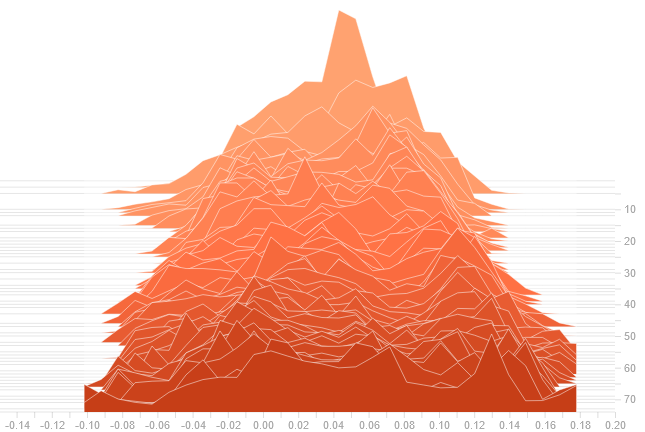
\includegraphics[width=1.0\linewidth]{Figures/LSTM-Bias.png}
    \end{minipage}\hfill
    \begin{minipage}{0.6\linewidth}
        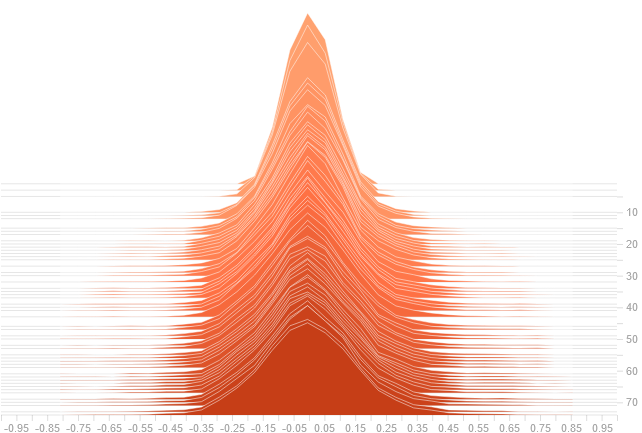
\includegraphics[width=1.0\linewidth]{Figures/LSTM-Weights.png}
    \end{minipage}
\end{figure}

The model training, validation and error comparison with previous model performances took approximately 3 minutes, after which the model predicted the subsequent day's forecast. Figure \ref{fig:lstm-final-data} shows how this looked. The forecaster accurately depicted the initial peaks for the entire day, including the morning, afternoon, and evening. It is clear however, that the rest of the data points may not be as accurate. This is not a significant drawback for the hybrid model, as the reactive algorithm is capable of making minor adjustments to the resources, ensuring that the SLA compliance is maintained.

\begin{comment}
\begin{figure}[htb]
    \centering
    \caption{Example of the forecasted workload}
    \label{fig:lstm-final-data}
    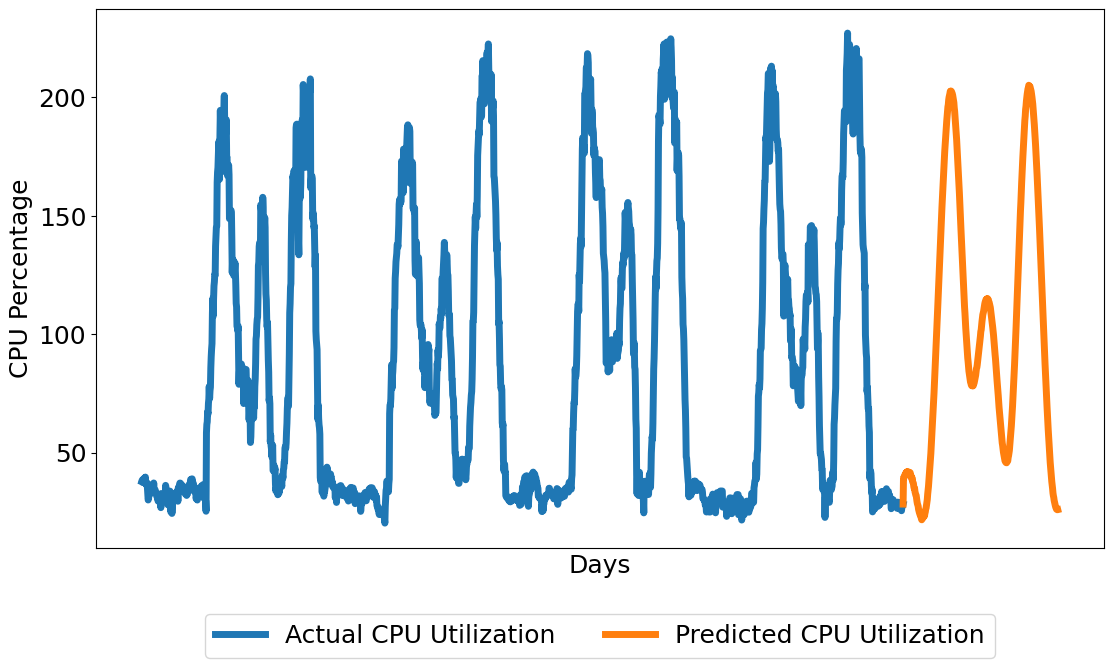
\includegraphics[width=1.0\linewidth]{Figures/LSTM-Final-Data.png}
\end{figure}
\end{comment}

\begin{center}
\begin{minipage}{\linewidth}
    \captionof{figure}{Example of the historical and forecast workload}
    \label{fig:lstm-final-data}
    \begin{tikzpicture}
        \begin{axis}[
            height=0.4\linewidth,
            width=\linewidth,
            xmin=-150,
            xmax=2460,  % Make xmax 150 above the final xtick
            ymin=0,
            ymajorgrids=true,
            yminorgrids=true,
            xmajorgrids=true,
            xminorgrids=true,
            grid style=dashed,
            xlabel={Time (Days)},
            ylabel={CPU Usage (\%)},
            legend style={at={(0.5,-0.3)},anchor=north,legend columns=-1},
            xticklabels={Day 1, Day 2, Day 3, Day 4, Day 5},
            xtick={462, 924, 1386, 1848, 2310}
        ]
            \addplot+[blue, mark=none] table [x=xtick, y=value, col sep=comma] {Data/LSTM-Final-Data-Value.csv};
            \addplot+[RedOrange, mark=none] table [x=xtick, y=value, col sep=comma] {Data/LSTM-Final-Data-Forecast.csv};
            %\draw[red, thick, dashed] (axis cs:0, 150) -- (axis cs:2472, 150);
            \legend{Historical, Forecast}
            %\addlegendimage{line width=0.3mm, dashed, color=red}
            %\addlegendentry{Threshold}
        \end{axis}
    \end{tikzpicture}
\end{minipage}
\end{center}

\subsection{Autoscaler Controller}
\label{subsec:ch4-auto-daemon-subsection}

The autoscaler controller stored a maximum of seven days of data for use by the proactive forecaster. Data that is too old is not very useful for a time-series model training on semi-predictable data \cite{greff2016lstm}, and only increases training time without adding much to the accuracy. This data was refreshed once every day to ensure that the latest data was always available to the hybrid autoscalers before training. Since training only took place once a day, the costly metric scraping operations done by the controller from the cloud layer could be reduced, thereby reducing the overall load on the network.\par

The controller sent a training request to the proactive autoscaler once every night. The time is chosen so that, due to the comparatively low amounts of user requests, the training process would be able to claim as much of the edge resources as possible without affecting the network availability. However, before sending the request, the controller computed whether or not an SLA violation took place in the past 24 hours. If it detected a violation, it assumed that the forecaster had not learnt enough of the time-series features to make an accurate prediction. This could be due to a variety of reasons such as lack of training data or conservative parameter values. To counteract this, the controller performed the following corrections:

\begin{itemize}
    \item $learning\_rate$ was decreased by 0.0005, to a minimum value of 0.002.
    \item $epochs$ was increased by 5, to a maximum of 100.
    \item $batch\_size$ was increased by 10, to a maximum of 200.
    \item $early\_stop$ threshold was increased by 5, to a maximum of 25.
\end{itemize}

The assumption here was that the training accuracy could be jump started by sacrificing short training times for one duration to better learn the time series features and thus reduce SLA violations. As long as SLA violations occur, these modifications keep being performed up until their configured limits. Experimental testing demonstrated that, at the most extreme hyper-parameter configuration, the training time increased to 10 minutes. Once no SLA violations were detected during a 24 hour time window, the hyper-parameters were reverted back to the default values. Doing so did not cause the model to lose any previous optimizations or reduce prediction accuracy, but had the added benefit of reducing training time and resources once again.